% Options for packages loaded elsewhere
\PassOptionsToPackage{unicode}{hyperref}
\PassOptionsToPackage{hyphens}{url}
%
\documentclass[
  12 pt,
  a4paper,
]{article}
\usepackage{amsmath,amssymb}
\usepackage{setspace}
\usepackage{iftex}
\ifPDFTeX
  \usepackage[T1]{fontenc}
  \usepackage[utf8]{inputenc}
  \usepackage{textcomp} % provide euro and other symbols
\else % if luatex or xetex
  \usepackage{unicode-math} % this also loads fontspec
  \defaultfontfeatures{Scale=MatchLowercase}
  \defaultfontfeatures[\rmfamily]{Ligatures=TeX,Scale=1}
\fi
\usepackage{lmodern}
\ifPDFTeX\else
  % xetex/luatex font selection
  \setmainfont[]{Times New Roman}
\fi
% Use upquote if available, for straight quotes in verbatim environments
\IfFileExists{upquote.sty}{\usepackage{upquote}}{}
\IfFileExists{microtype.sty}{% use microtype if available
  \usepackage[]{microtype}
  \UseMicrotypeSet[protrusion]{basicmath} % disable protrusion for tt fonts
}{}
\makeatletter
\@ifundefined{KOMAClassName}{% if non-KOMA class
  \IfFileExists{parskip.sty}{%
    \usepackage{parskip}
  }{% else
    \setlength{\parindent}{0pt}
    \setlength{\parskip}{6pt plus 2pt minus 1pt}}
}{% if KOMA class
  \KOMAoptions{parskip=half}}
\makeatother
\usepackage{xcolor}
\usepackage[margin=1in]{geometry}
\usepackage{color}
\usepackage{fancyvrb}
\newcommand{\VerbBar}{|}
\newcommand{\VERB}{\Verb[commandchars=\\\{\}]}
\DefineVerbatimEnvironment{Highlighting}{Verbatim}{commandchars=\\\{\}}
% Add ',fontsize=\small' for more characters per line
\usepackage{framed}
\definecolor{shadecolor}{RGB}{248,248,248}
\newenvironment{Shaded}{\begin{snugshade}}{\end{snugshade}}
\newcommand{\AlertTok}[1]{\textcolor[rgb]{0.94,0.16,0.16}{#1}}
\newcommand{\AnnotationTok}[1]{\textcolor[rgb]{0.56,0.35,0.01}{\textbf{\textit{#1}}}}
\newcommand{\AttributeTok}[1]{\textcolor[rgb]{0.13,0.29,0.53}{#1}}
\newcommand{\BaseNTok}[1]{\textcolor[rgb]{0.00,0.00,0.81}{#1}}
\newcommand{\BuiltInTok}[1]{#1}
\newcommand{\CharTok}[1]{\textcolor[rgb]{0.31,0.60,0.02}{#1}}
\newcommand{\CommentTok}[1]{\textcolor[rgb]{0.56,0.35,0.01}{\textit{#1}}}
\newcommand{\CommentVarTok}[1]{\textcolor[rgb]{0.56,0.35,0.01}{\textbf{\textit{#1}}}}
\newcommand{\ConstantTok}[1]{\textcolor[rgb]{0.56,0.35,0.01}{#1}}
\newcommand{\ControlFlowTok}[1]{\textcolor[rgb]{0.13,0.29,0.53}{\textbf{#1}}}
\newcommand{\DataTypeTok}[1]{\textcolor[rgb]{0.13,0.29,0.53}{#1}}
\newcommand{\DecValTok}[1]{\textcolor[rgb]{0.00,0.00,0.81}{#1}}
\newcommand{\DocumentationTok}[1]{\textcolor[rgb]{0.56,0.35,0.01}{\textbf{\textit{#1}}}}
\newcommand{\ErrorTok}[1]{\textcolor[rgb]{0.64,0.00,0.00}{\textbf{#1}}}
\newcommand{\ExtensionTok}[1]{#1}
\newcommand{\FloatTok}[1]{\textcolor[rgb]{0.00,0.00,0.81}{#1}}
\newcommand{\FunctionTok}[1]{\textcolor[rgb]{0.13,0.29,0.53}{\textbf{#1}}}
\newcommand{\ImportTok}[1]{#1}
\newcommand{\InformationTok}[1]{\textcolor[rgb]{0.56,0.35,0.01}{\textbf{\textit{#1}}}}
\newcommand{\KeywordTok}[1]{\textcolor[rgb]{0.13,0.29,0.53}{\textbf{#1}}}
\newcommand{\NormalTok}[1]{#1}
\newcommand{\OperatorTok}[1]{\textcolor[rgb]{0.81,0.36,0.00}{\textbf{#1}}}
\newcommand{\OtherTok}[1]{\textcolor[rgb]{0.56,0.35,0.01}{#1}}
\newcommand{\PreprocessorTok}[1]{\textcolor[rgb]{0.56,0.35,0.01}{\textit{#1}}}
\newcommand{\RegionMarkerTok}[1]{#1}
\newcommand{\SpecialCharTok}[1]{\textcolor[rgb]{0.81,0.36,0.00}{\textbf{#1}}}
\newcommand{\SpecialStringTok}[1]{\textcolor[rgb]{0.31,0.60,0.02}{#1}}
\newcommand{\StringTok}[1]{\textcolor[rgb]{0.31,0.60,0.02}{#1}}
\newcommand{\VariableTok}[1]{\textcolor[rgb]{0.00,0.00,0.00}{#1}}
\newcommand{\VerbatimStringTok}[1]{\textcolor[rgb]{0.31,0.60,0.02}{#1}}
\newcommand{\WarningTok}[1]{\textcolor[rgb]{0.56,0.35,0.01}{\textbf{\textit{#1}}}}
\usepackage{longtable,booktabs,array}
\usepackage{calc} % for calculating minipage widths
% Correct order of tables after \paragraph or \subparagraph
\usepackage{etoolbox}
\makeatletter
\patchcmd\longtable{\par}{\if@noskipsec\mbox{}\fi\par}{}{}
\makeatother
% Allow footnotes in longtable head/foot
\IfFileExists{footnotehyper.sty}{\usepackage{footnotehyper}}{\usepackage{footnote}}
\makesavenoteenv{longtable}
\usepackage{graphicx}
\makeatletter
\def\maxwidth{\ifdim\Gin@nat@width>\linewidth\linewidth\else\Gin@nat@width\fi}
\def\maxheight{\ifdim\Gin@nat@height>\textheight\textheight\else\Gin@nat@height\fi}
\makeatother
% Scale images if necessary, so that they will not overflow the page
% margins by default, and it is still possible to overwrite the defaults
% using explicit options in \includegraphics[width, height, ...]{}
\setkeys{Gin}{width=\maxwidth,height=\maxheight,keepaspectratio}
% Set default figure placement to htbp
\makeatletter
\def\fps@figure{htbp}
\makeatother
\setlength{\emergencystretch}{3em} % prevent overfull lines
\providecommand{\tightlist}{%
  \setlength{\itemsep}{0pt}\setlength{\parskip}{0pt}}
\setcounter{secnumdepth}{-\maxdimen} % remove section numbering
\ifLuaTeX
\usepackage[bidi=basic]{babel}
\else
\usepackage[bidi=default]{babel}
\fi
\babelprovide[main,import]{spanish}
\ifPDFTeX
\else
\babelfont[spanish]{rm}{Times New Roman}
\fi
% get rid of language-specific shorthands (see #6817):
\let\LanguageShortHands\languageshorthands
\def\languageshorthands#1{}
\ifLuaTeX
  \usepackage{selnolig}  % disable illegal ligatures
\fi
\IfFileExists{bookmark.sty}{\usepackage{bookmark}}{\usepackage{hyperref}}
\IfFileExists{xurl.sty}{\usepackage{xurl}}{} % add URL line breaks if available
\urlstyle{same}
\hypersetup{
  pdfauthor={Tomàs Ferrandis Moscardó},
  pdflang={es-ES},
  hidelinks,
  pdfcreator={LaTeX via pandoc}}

\title{ANÁLISIS UNIVARIABLE SOBRE PREFERENCIA DE PRESIDENTE/A DE
GOBIERNO SEGÚN BARÓMETRO DEL CIS DE JULIO 2023\\
(ESTUDIO 3415)}
\usepackage{etoolbox}
\makeatletter
\providecommand{\subtitle}[1]{% add subtitle to \maketitle
  \apptocmd{\@title}{\par {\large #1 \par}}{}{}
}
\makeatother
\subtitle{Técnicas de Investigación en Ciencia Política I. UBU\\
Práctica 1. Apartado 3}
\author{Tomàs Ferrandis Moscardó}
\date{2023-03-18}

\begin{document}
\maketitle

{
\setcounter{tocdepth}{2}
\tableofcontents
}
\setstretch{1.5}
\newpage
\renewcommand\tablename{Tabla}

\hypertarget{introducciuxf3n}{%
\section{1. INTRODUCCIÓN}\label{introducciuxf3n}}

Esta actividad corresponde al apartado 3º de la Práctica 1 de Técnicas
de Investigación en Ciencia Política I. Se trata de un \emph{análisis
univariado} sobre la variable PREFPTE del Barómetro del CIS de julio de
2023 (Estudio 3415). Concretamente se trata de la pregunta P8 que dice:
\emph{De los/las principales líderes políticos/as, ¿quién preferiría que
fuese el/la presidente/a del Gobierno tras las elecciones?} . Obviamente
al tratarse de análisis univariado solo puede ser descriptivo.

Para el análisis de los datos se usa el \textbf{lenguaje de programación
R}. Se incorpora el código en los documentos renderizados (HTML y PDF)
activando la opción \emph{echo} de los chunks (\emph{echo=TRUE}). En
algunos chunks no interesa la impresión del resultado por lo que se
configuran con \emph{results=`hide'}. Si se desea ver el resultado de la
ejecución correcta de alguno de estos chunks bastará con eliminar el
parametro \emph{results=`hide'} en el fichero Rmd descargado (ver
\protect\hyperlink{id-github}{punto 8} para descarga ).

\hypertarget{obtenciuxf3n-de-datos}{%
\section{2. OBTENCIÓN DE DATOS}\label{obtenciuxf3n-de-datos}}

\begin{Shaded}
\begin{Highlighting}[]
\FunctionTok{suppressMessages}\NormalTok{(\{ }\CommentTok{\# Suprimimos mensajes de salida al...}
\CommentTok{\# instalar paquetes (si no están) con las funciones...}
\ControlFlowTok{if}\NormalTok{(}\SpecialCharTok{!}\FunctionTok{require}\NormalTok{(haven))\{}\FunctionTok{install.packages}\NormalTok{(}\StringTok{"haven"}\NormalTok{)\} }\CommentTok{\# para abrir fichero .sav}
\ControlFlowTok{if}\NormalTok{(}\SpecialCharTok{!}\FunctionTok{require}\NormalTok{(epiDisplay))\{}\FunctionTok{install.packages}\NormalTok{(}\StringTok{"epiDisplay"}\NormalTok{)\} }\CommentTok{\# para gráfico }
\ControlFlowTok{if}\NormalTok{(}\SpecialCharTok{!}\FunctionTok{require}\NormalTok{(knitr))\{}\FunctionTok{install.packages}\NormalTok{(}\StringTok{"knitr"}\NormalTok{)\}}\CommentTok{\#tabla dinámica Rmd y otros}
\ControlFlowTok{if}\NormalTok{(}\SpecialCharTok{!}\FunctionTok{require}\NormalTok{(xlsx))\{}\FunctionTok{install.packages}\NormalTok{(}\StringTok{"xlsx"}\NormalTok{)\} }\CommentTok{\# manejo de ficheros .xlsx}
\NormalTok{\})}
\end{Highlighting}
\end{Shaded}

\hypertarget{fichero-y-datos-en-abierto}{%
\subsection{2.1 Fichero y Datos en
Abierto}\label{fichero-y-datos-en-abierto}}

Del portal del CIS, se localiza el \emph{barómetro de julio 2023} y se
descargan los datos estadísticos en un formato de fichero \emph{.sav}

Se usará una variable R (\emph{nombreFichero}) con la ruta relativa
\emph{DATOS} que será el directorio donde se guardará los ficheros de
datos.

\begin{Shaded}
\begin{Highlighting}[]
\CommentTok{\# El fichero .sav se guardará en una subcarpeta DATOS}
\NormalTok{nombreFichero}\OtherTok{\textless{}{-}}\StringTok{"datosjulio2023.sav"}
\NormalTok{directorioTrabajo}\OtherTok{\textless{}{-}}\FunctionTok{getwd}\NormalTok{()}
\NormalTok{rutaFichero}\OtherTok{\textless{}{-}}\FunctionTok{paste}\NormalTok{(directorioTrabajo,}\StringTok{"DATOS"}\NormalTok{,nombreFichero,}\AttributeTok{sep=}\StringTok{"/"}\NormalTok{)}
\end{Highlighting}
\end{Shaded}

\hypertarget{creaciuxf3n-de-la-base-de-datos-data-frame}{%
\subsection{\texorpdfstring{2.2 Creación de la base de datos (\emph{data
frame})}{2.2 Creación de la base de datos (data frame)}}\label{creaciuxf3n-de-la-base-de-datos-data-frame}}

A partir del fichero de tipo \emph{sav} se creará el objeto \emph{data
frame} de R. Este data frame será la base de datos inicial con todos los
datos obtenidos de la muestra mediante la encuesta.

\begin{Shaded}
\begin{Highlighting}[]
\NormalTok{df\_cisjulio}\OtherTok{\textless{}{-}}\FunctionTok{read\_sav}\NormalTok{(rutaFichero)}
\end{Highlighting}
\end{Shaded}

\hypertarget{consultar-el-cuestionario-y-el-diccionario-de-datos}{%
\subsection{2.3 Consultar el cuestionario y el diccionario de
datos}\label{consultar-el-cuestionario-y-el-diccionario-de-datos}}

Observando el cuestionario del CIS se puede ver qué se trata de una
variable de tipo cualitativa. Una comprobación que se puede hacer
mediante R es ver que los valores existentes en la base de datos
coinciden coherentemente con las respuestas válidas del cuestionario.
Mediante la función \emph{unique} devuelve todos valores existentes en
la columna sin duplicados, además de un listado de los valores posibles
y sus respectiva etiquetas definidos. Puede ser de gran ayuda para esta
comprobación.

\begin{Shaded}
\begin{Highlighting}[]
\FunctionTok{unique}\NormalTok{(df\_cisjulio}\SpecialCharTok{$}\NormalTok{PREFPTE) }\CommentTok{\# obtiene los valores sin duplicado }
\end{Highlighting}
\end{Shaded}

\hypertarget{tipo-de-variable-prefpte}{%
\subsection{2.4 Tipo de variable
PREFPTE}\label{tipo-de-variable-prefpte}}

A la vista de los resultados anteriores y, tras leer la documentación
del cuestionario, se puede deducir que la variable PREFTE es una
variable \emph{cualitativa nominal} con escasos valores como es habitual
(11) y, donde cada uno de ellos tiene una etiqueta asociada.

Antes de obtener medidas de posición o de variación se deberá tratar
previamente la matriz de datos.

\newpage

\hypertarget{preparaciuxf3n-de-la-matriz-de-datos}{%
\section{3. PREPARACIÓN DE LA MATRIZ DE
DATOS}\label{preparaciuxf3n-de-la-matriz-de-datos}}

A partir de la matriz obtenida se procederá a limpiar y simplificar esta
base de datos inicial.

\hypertarget{limpieza-de-la-base-de-datos}{%
\subsection{3.1 Limpieza de la base de
datos}\label{limpieza-de-la-base-de-datos}}

\hypertarget{reducciuxf3n-del-tamauxf1o-de-la-matriz-de-datos}{%
\subsubsection{Reducción del tamaño de la matriz de
datos}\label{reducciuxf3n-del-tamauxf1o-de-la-matriz-de-datos}}

Al tratarse de un \emph{análisis univariado} en que solo se va a
considerar una columna es conveniente prescindir de los demás datos
usando así, un \emph{data frame} de menor tamaño (menos columnas) y más
simple.

\begin{Shaded}
\begin{Highlighting}[]
\NormalTok{df\_cis}\OtherTok{\textless{}{-}}\NormalTok{df\_cisjulio [, }\StringTok{"PREFPTE"}\NormalTok{]}
\end{Highlighting}
\end{Shaded}

Para comprobar el resultado se puede usar instrucciones de lectura del
data frame de R como \emph{head} o \emph{tail}.

\begin{Shaded}
\begin{Highlighting}[]
\FunctionTok{tail}\NormalTok{(df\_cis,}\DecValTok{4}\NormalTok{) }\CommentTok{\# Muestra los 4 últimos casos}
\FunctionTok{head}\NormalTok{(df\_cis,}\DecValTok{4}\NormalTok{) }\CommentTok{\# Muestra los 4 primeros casos}
\end{Highlighting}
\end{Shaded}

Otra comprobación interesante consiste en comparar las dimensiones de
ambos \emph{data frames}, el inicial y el resumido, con funciones de R
como:

\begin{itemize}
\tightlist
\item
  \emph{dim()} Devuelve un vector con dos valores: el número total de
  casos (lineas del \emph{data frame}) y el número de variables
  (columnas del \emph{data frame}).
\item
  \emph{nrow()} Devuelve el número total de casos (lineas del \emph{data
  frame})
\item
  \emph{ncols()} el número de variables (columnas del \emph{data frame})
\end{itemize}

\begin{Shaded}
\begin{Highlighting}[]
\FunctionTok{dim}\NormalTok{(df\_cis)}
\FunctionTok{dim}\NormalTok{(df\_cisjulio)}
\FunctionTok{nrow}\NormalTok{(df\_cis)}
\FunctionTok{nrow}\NormalTok{(df\_cisjulio)}
\FunctionTok{ncol}\NormalTok{(df\_cisjulio)}

\NormalTok{n}\OtherTok{\textless{}{-}}\FunctionTok{nrow}\NormalTok{(df\_cis) }\CommentTok{\# La n del muestreo}
\end{Highlighting}
\end{Shaded}

Lógicamente el número de casos es 8798 en ambos \emph{data frames}.

\begin{quote}
8798 es el valor \textbf{n} del muestreo
\end{quote}

\hypertarget{recodificaciuxf3n}{%
\subsection{3.2 Recodificación}\label{recodificaciuxf3n}}

\hypertarget{duplicaciuxf3n-de-la-variable}{%
\subsubsection{Duplicación de la
variable}\label{duplicaciuxf3n-de-la-variable}}

Lo más prudente cuando se va a editar datos es que estos se realicen
sobre una copia. Por esta razón duplicaremos la columna del \emph{data
frame}

\begin{Shaded}
\begin{Highlighting}[]
\NormalTok{df\_cis}\SpecialCharTok{$}\NormalTok{recPREFPTE}\OtherTok{\textless{}{-}}\NormalTok{df\_cis}\SpecialCharTok{$}\NormalTok{PREFPTE}
\end{Highlighting}
\end{Shaded}

\hypertarget{valores-vuxe1lidos-y-no-vuxe1lidos}{%
\subsubsection{Valores válidos y no
válidos}\label{valores-vuxe1lidos-y-no-vuxe1lidos}}

Una vez examinados los datos en el apartado 3.2 anterior, ya se puede
decidir qué valores de la variable son válidos y cuales no interesan
para nuestro análisis.

\emph{Valores válidos: niveles y etiquetas}

\begin{itemize}
\tightlist
\item
  Pedro Sánchez 1
\item
  Alberto Núñez Feijóo 2
\item
  Santiago Abascal 3
\item
  Yolanda Díaz 4
\item
  Ione Belarra 10
\item
  Íñigo Errejón 7
\item
  Isabel Díaz Ayuso 8
\end{itemize}

\emph{Valores no válidos: niveles y etiquetas}

\begin{itemize}
\tightlist
\item
  (O LEER) Ninguno/a de ellos/as 97
\item
  (NO LEER) Otro/a 96
\item
  N.S. 98
\item
  N.C. 99
\end{itemize}

Se deberá agrupar bajo la etiqueta de NA (valor ausente) los valores 96,
97, 98 y 99. Para ello, antes se duplicará esta columna, es decir, se
insertará dentro del \emph{data frame} una segunda columna con los
mismos valores. Sobre esta columna se editarán los datos
(\textbf{recodificación}).

\hypertarget{agrupaciuxf3n-de-valores-no-vuxe1lidos}{%
\subsubsection{Agrupación de valores NO
válidos}\label{agrupaciuxf3n-de-valores-no-vuxe1lidos}}

Todos los valores que no son válidos para el análisis (96, 97, 98, 99 se
actualizarán a NA.

Al mismo tiempo se puede simplificar el resto de valores en este caso,
solo cambiándolos a {[}1,2,3,4,5,6 7{]}.

\begin{Shaded}
\begin{Highlighting}[]
\NormalTok{df\_cis0}\OtherTok{\textless{}{-}}\NormalTok{df\_cis}
\NormalTok{df\_cis}\SpecialCharTok{$}\NormalTok{recPREFPTE[df\_cis}\SpecialCharTok{$}\NormalTok{recPREFPTE }\SpecialCharTok{\textgreater{}=}\DecValTok{96}\NormalTok{]}\OtherTok{\textless{}{-}}\ConstantTok{NA}
\NormalTok{df\_cis}\SpecialCharTok{$}\NormalTok{recPREFPTE}\OtherTok{\textless{}{-}}\FunctionTok{factor}\NormalTok{(df\_cis}\SpecialCharTok{$}\NormalTok{recPREFPTE,}
                  \AttributeTok{levels=}\FunctionTok{c}\NormalTok{(}\DecValTok{1}\NormalTok{,}\DecValTok{2}\NormalTok{,}\DecValTok{3}\NormalTok{,}\DecValTok{4}\NormalTok{,}\DecValTok{5}\NormalTok{,}\DecValTok{6}\NormalTok{,}\DecValTok{7}\NormalTok{),}
                  \AttributeTok{labels=}\FunctionTok{c}\NormalTok{(}\StringTok{"Pedro Sánchez"}\NormalTok{, }\StringTok{"Alberto Núñez Feijóo"}\NormalTok{,}
                   \StringTok{"Santiago Abascal"}\NormalTok{,}\StringTok{"Yolanda Díaz"}\NormalTok{,}\StringTok{"Ione Belarra"}\NormalTok{,}
                   \StringTok{"Íñigo Errejón"}\NormalTok{,}\StringTok{"Isabel Díaz Ayuso"}\NormalTok{))}
\end{Highlighting}
\end{Shaded}

El tratamiento de los valores no válidos es doble. Se excluirán del
análisis pero se deberá valorar su importancia. Para ello se debe ver su
peso en relación al conjunto de valores. En R tenemos la función
\emph{summary} que devuelve los valores de posición central (media,
mediana y moda) y los cuartiles. Se puede parametrizar para que cuente
también los valores NA (remove missing values = FALSE)

\begin{Shaded}
\begin{Highlighting}[]
\NormalTok{numero\_na}\OtherTok{\textless{}{-}}\FunctionTok{sum}\NormalTok{(}\FunctionTok{is.na}\NormalTok{(df\_cis}\SpecialCharTok{$}\NormalTok{recPREFPTE)) }\CommentTok{\# Guarda valor en variable para...}
\NormalTok{porcentaje\_na}\OtherTok{\textless{}{-}}\FunctionTok{round}\NormalTok{(}\FunctionTok{mean}\NormalTok{(}\FunctionTok{is.na}\NormalTok{(df\_cis}\SpecialCharTok{$}\NormalTok{recPREFPTE))}\SpecialCharTok{*}\DecValTok{100}\NormalTok{,}\DecValTok{1}\NormalTok{) }\CommentTok{\#calcular \% NA}
\end{Highlighting}
\end{Shaded}

\begin{Shaded}
\begin{Highlighting}[]
\CommentTok{\# Totaliza por valores, incluyendo NA)}
\FunctionTok{kable}\NormalTok{(}\FunctionTok{summary}\NormalTok{(df\_cis}\SpecialCharTok{$}\NormalTok{recPREFPTE, }\AttributeTok{na.rm=}\ConstantTok{FALSE}\NormalTok{), }
      \AttributeTok{col.names =} \FunctionTok{c}\NormalTok{(}\StringTok{"Líder"}\NormalTok{,}\StringTok{"Repeticiones"}\NormalTok{),}\AttributeTok{caption=}\StringTok{"Summary"}\NormalTok{)}
\end{Highlighting}
\end{Shaded}

\begin{longtable}[]{@{}lr@{}}
\caption{Summary}\tabularnewline
\toprule\noalign{}
Líder & Repeticiones \\
\midrule\noalign{}
\endfirsthead
\toprule\noalign{}
Líder & Repeticiones \\
\midrule\noalign{}
\endhead
\bottomrule\noalign{}
\endlastfoot
Pedro Sánchez & 2631 \\
Alberto Núñez Feijóo & 2576 \\
Santiago Abascal & 658 \\
Yolanda Díaz & 1300 \\
Ione Belarra & 0 \\
Íñigo Errejón & 0 \\
Isabel Díaz Ayuso & 8 \\
NA's & 1625 \\
\end{longtable}

\emph{Importancia de los valores perdidos NA}

Hay un total de 1625 lo que supone un porcentaje del 18.5 de casos no
válidos sobre el total de n=8798.

\newpage

\hypertarget{medidas-de-tendencia-central}{%
\section{4 MEDIDAS DE TENDENCIA
CENTRAL}\label{medidas-de-tendencia-central}}

Al tratarse de una variable \textbf{cualitativa nominal} solo tiene
sentido como medida de tendencia central la \emph{moda}. La
\emph{mediana} y la \emph{media}, no.

\hypertarget{moda}{%
\subsection{4.1 Moda}\label{moda}}

Para el cálculo de la moda, R no dispone de ninguna función en sus
librerías, se puede usar una función de usuario como la aportada en los
apuntes de la asignatura.

\emph{Función Moda}

\begin{Shaded}
\begin{Highlighting}[]
\NormalTok{moda }\OtherTok{\textless{}{-}} \ControlFlowTok{function}\NormalTok{(v) \{}
\NormalTok{  uniqv }\OtherTok{\textless{}{-}} \FunctionTok{unique}\NormalTok{(v)}
\NormalTok{  uniqv[}\FunctionTok{which.max}\NormalTok{(}\FunctionTok{tabulate}\NormalTok{(}\FunctionTok{match}\NormalTok{(v, uniqv)))]}
\NormalTok{\}}
\end{Highlighting}
\end{Shaded}

Una vez creada la función e incorporado su código en el documento
RMarkdown (o script R) se podrá llamar y almacenar su resultado en una
variable para consultas u operaciones posteriores.

\begin{Shaded}
\begin{Highlighting}[]
\NormalTok{varModa}\OtherTok{\textless{}{-}}\FunctionTok{moda}\NormalTok{(df\_cis}\SpecialCharTok{$}\NormalTok{recPREFPTE) }\CommentTok{\#llama a la función y recupera valor}
\end{Highlighting}
\end{Shaded}

La moda es: \emph{Pedro Sánchez}

\newpage

\hypertarget{medidas-de-dispersiuxf3n-central}{%
\section{5. MEDIDAS DE DISPERSIÓN
CENTRAL}\label{medidas-de-dispersiuxf3n-central}}

Al tratarse de una variable cualitativa nominal no tiene sentido
estudiar un comportamiento en la distribución de valores.

\hypertarget{tabla-de-frecuencias-de-preferencia-de-presidentea}{%
\subsection{5.1 Tabla de frecuencias de Preferencia de
presidente/a}\label{tabla-de-frecuencias-de-preferencia-de-presidentea}}

En los siguientes análisis de datos se excluirán los valores no válidos.

\hypertarget{frecuencias-absolutas}{%
\subsubsection{Frecuencias absolutas}\label{frecuencias-absolutas}}

La frecuencia absoluta indica la suma de casos que se deciden por cada
uno de los candidatos.

\begin{Shaded}
\begin{Highlighting}[]
\CommentTok{\# La función *table* de R puede ignorar o no los NA (useNA="no"/"ifany")}
\CommentTok{\# por defecto. useNA="no" (los ignora, no haría falta indicarlo)}


\CommentTok{\# table(df\_cis$recPREFPTE, useNA="no") \# En R estrictamente}

\CommentTok{\# Uso de formato RMarkdown }
\FunctionTok{kable}\NormalTok{(}\FunctionTok{table}\NormalTok{(df\_cis}\SpecialCharTok{$}\NormalTok{recPREFPTE),}\AttributeTok{column.width=}\FunctionTok{c}\NormalTok{(}\StringTok{"30\%"}\NormalTok{,}\StringTok{"70\%"}\NormalTok{),}
  \AttributeTok{col.names =} \FunctionTok{c}\NormalTok{(}\StringTok{"Líder"}\NormalTok{,}\StringTok{"Repeticiones"}\NormalTok{),}\AttributeTok{caption=}\StringTok{"Frecuencia absoluta"}\NormalTok{)}
\end{Highlighting}
\end{Shaded}

\begin{longtable}[]{@{}lr@{}}
\caption{Frecuencia absoluta}\tabularnewline
\toprule\noalign{}
Líder & Repeticiones \\
\midrule\noalign{}
\endfirsthead
\toprule\noalign{}
Líder & Repeticiones \\
\midrule\noalign{}
\endhead
\bottomrule\noalign{}
\endlastfoot
Pedro Sánchez & 2631 \\
Alberto Núñez Feijóo & 2576 \\
Santiago Abascal & 658 \\
Yolanda Díaz & 1300 \\
Ione Belarra & 0 \\
Íñigo Errejón & 0 \\
Isabel Díaz Ayuso & 8 \\
\end{longtable}

\hypertarget{frecuencias-relativas.}{%
\subsubsection{Frecuencias relativas.}\label{frecuencias-relativas.}}

La frecuencia relativa indica el porcentaje respecto al total de casos
de los valores del apartado anterior. Es decir, el porcentaje de casos
que se prefieren a cada candidato.

\begin{Shaded}
\begin{Highlighting}[]
\FunctionTok{kable}\NormalTok{(}\FunctionTok{round}\NormalTok{(}\FunctionTok{prop.table}\NormalTok{(}\FunctionTok{table}\NormalTok{(df\_cis}\SpecialCharTok{$}\NormalTok{recPREFPTE,}\AttributeTok{useNA=}\StringTok{"no"}\NormalTok{))}\SpecialCharTok{*}\DecValTok{100}\NormalTok{,}\AttributeTok{digits=}\DecValTok{1}\NormalTok{),}
      \AttributeTok{col.names =} \FunctionTok{c}\NormalTok{(}\StringTok{"Líder"}\NormalTok{,}\StringTok{"\% de repeticiones"}\NormalTok{),}\AttributeTok{caption=}\StringTok{"Frecuencia relativa"}\NormalTok{)}
\end{Highlighting}
\end{Shaded}

\begin{longtable}[]{@{}lr@{}}
\caption{Frecuencia relativa}\tabularnewline
\toprule\noalign{}
Líder & \% de repeticiones \\
\midrule\noalign{}
\endfirsthead
\toprule\noalign{}
Líder & \% de repeticiones \\
\midrule\noalign{}
\endhead
\bottomrule\noalign{}
\endlastfoot
Pedro Sánchez & 36.7 \\
Alberto Núñez Feijóo & 35.9 \\
Santiago Abascal & 9.2 \\
Yolanda Díaz & 18.1 \\
Ione Belarra & 0.0 \\
Íñigo Errejón & 0.0 \\
Isabel Díaz Ayuso & 0.1 \\
\end{longtable}

\begin{itemize}
\tightlist
\item
  La función \emph{table} de R devolverá el total de casos de cada
  valor. \emph{Ejemplo: Pedro Sánchez: 2731}
\item
  La función \emph{prop} devolverá el tanto x 1 del valor anterior.
  \emph{Ejemplo: Pedro Sánchez: 0,361}
\item
  Se multiplicará x 100 para obtener el porcentaje.
\item
  Con la función aritmética \emph{round} se redondeará a 1 decimal como
  es habitual en Ciencias Sociales.
\end{itemize}

\newpage

\hypertarget{gruxe1ficos}{%
\section{6 Gráficos}\label{gruxe1ficos}}

Para variables nominales, se puede optar por:

\begin{itemize}
\tightlist
\item
  Gráfico de barras
\item
  Gráfico de sectores
\item
  Gráfico de Pareto
\end{itemize}

En los siguientes subapartados ser verán los resultados en las
diferentes opciones.

\hypertarget{gruxe1fico-de-barras}{%
\subsection{6.1 Gráfico de barras}\label{gruxe1fico-de-barras}}

Para una variable nominal como es el caso, el gráfico más adecuado es el
diagrama de barras.

\begin{Shaded}
\begin{Highlighting}[]
\CommentTok{\# Se adoptan los colores identificativos de la opción política}
\NormalTok{colores}\OtherTok{\textless{}{-}}\FunctionTok{c}\NormalTok{(}\StringTok{"red"}\NormalTok{,}\StringTok{"blue"}\NormalTok{,}\StringTok{"\#FF33FF"}\NormalTok{,}\StringTok{"\#2ecc71"}\NormalTok{,}\StringTok{"\#2980b9"}\NormalTok{,}\StringTok{"\#ab47bc"}\NormalTok{,}\StringTok{"\#c8e6c9"}\NormalTok{)}
\NormalTok{coloresInvertidos}\OtherTok{\textless{}{-}}\FunctionTok{rev}\NormalTok{(colores)}
\NormalTok{grafico }\OtherTok{\textless{}{-}} \FunctionTok{tab1}\NormalTok{(df\_cis}\SpecialCharTok{$}\NormalTok{recPREFPTE,}\AttributeTok{cum.percent =} \ConstantTok{TRUE}\NormalTok{,}
                \AttributeTok{sort.group=}\StringTok{"decreasing"}\NormalTok{,}\AttributeTok{xlab=}\StringTok{"\% preferencia"}\NormalTok{,}
                \AttributeTok{decimal=}\DecValTok{1}\NormalTok{,}\AttributeTok{bar.values =} \StringTok{"percent"}\NormalTok{,  }
                \AttributeTok{main=}\StringTok{"Gráfico 1. Preferencia Presidencia de Gobierno"}\NormalTok{,}
                \AttributeTok{col=}\NormalTok{coloresInvertidos, }\AttributeTok{missing =} \ConstantTok{FALSE}\NormalTok{)}
\end{Highlighting}
\end{Shaded}

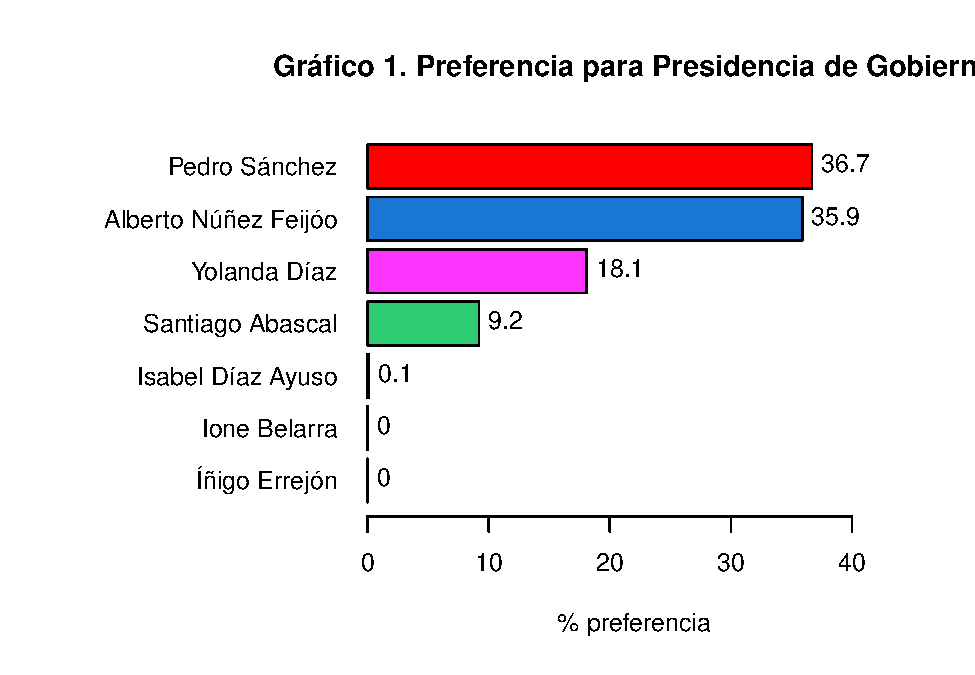
\includegraphics{preferenciaPte_files/figure-latex/grafico-1.pdf}
\newpage

\hypertarget{gruxe1fico-de-sectores}{%
\subsection{6.2 Gráfico de sectores}\label{gruxe1fico-de-sectores}}

Alternativamente se podría usar el gráfico de sectores.

\begin{Shaded}
\begin{Highlighting}[]
\NormalTok{valores}\OtherTok{\textless{}{-}}\FunctionTok{as.numeric}\NormalTok{(}\FunctionTok{round}\NormalTok{(}\FunctionTok{prop.table}\NormalTok{(}\FunctionTok{table}\NormalTok{(df\_cis}\SpecialCharTok{$}\NormalTok{recPREFPTE))}\SpecialCharTok{*}\DecValTok{100}\NormalTok{,}
                                                              \AttributeTok{digits=}\DecValTok{1}\NormalTok{))}
\NormalTok{nombres}\OtherTok{\textless{}{-}}\FunctionTok{names}\NormalTok{(}\FunctionTok{round}\NormalTok{(}\FunctionTok{prop.table}\NormalTok{(}\FunctionTok{table}\NormalTok{(df\_cis}\SpecialCharTok{$}\NormalTok{recPREFPTE))}\SpecialCharTok{*}\DecValTok{100}\NormalTok{,}\AttributeTok{digits=}\DecValTok{1}\NormalTok{))}
\CommentTok{\#vector con los índices ordenados según valor decreciente}
\NormalTok{orden}\OtherTok{\textless{}{-}}\FunctionTok{order}\NormalTok{(valores,}\AttributeTok{decreasing=}\ConstantTok{TRUE}\NormalTok{)}
\NormalTok{valoresOrdenados}\OtherTok{\textless{}{-}}\NormalTok{valores[orden]}
\NormalTok{nombresOrdenados}\OtherTok{\textless{}{-}}\NormalTok{nombres[orden]}
\FunctionTok{pie}\NormalTok{(valores, }\AttributeTok{labels =}\NormalTok{ nombres, }
    \AttributeTok{main =} \StringTok{"Gráfico 2. Preferencia para Presidencia de Gobierno"}\NormalTok{,}
    \AttributeTok{col =}\NormalTok{ colores, }\AttributeTok{cex=}\FloatTok{0.8}\NormalTok{)}
\end{Highlighting}
\end{Shaded}

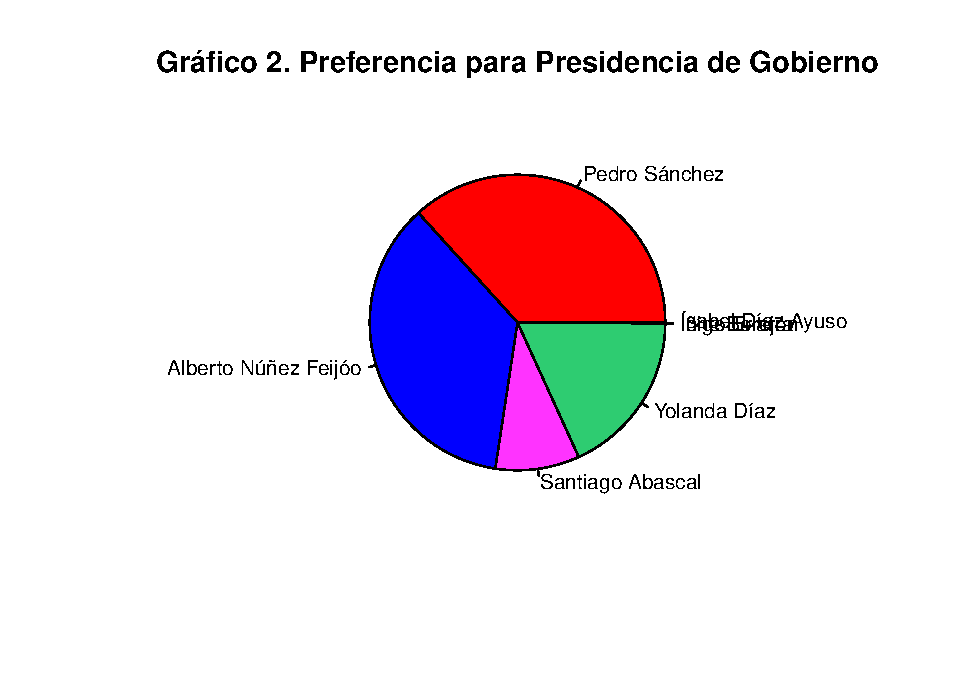
\includegraphics{preferenciaPte_files/figure-latex/graficoPIE-1.pdf}

Como se puede observar, el gráfico de sectores no muestra con la misma
claridad los porcentajes que el gráfico de barras.

\hypertarget{gruxe1fico-de-pareto}{%
\subsection{6.3 Gráfico de Pareto}\label{gruxe1fico-de-pareto}}

Esta otra alternativa ordena los datos y las frecuencias en sentido
decreciente y muestra qué porcentaje acumulan en total las opciones
representadas.

\begin{Shaded}
\begin{Highlighting}[]
\NormalTok{valores}\OtherTok{\textless{}{-}}\FunctionTok{as.numeric}\NormalTok{(}\FunctionTok{round}\NormalTok{(}\FunctionTok{prop.table}\NormalTok{(}\FunctionTok{table}\NormalTok{(df\_cis}\SpecialCharTok{$}\NormalTok{recPREFPTE))}\SpecialCharTok{*}\DecValTok{100}\NormalTok{,}
                                                              \AttributeTok{digits=}\DecValTok{1}\NormalTok{))}
\NormalTok{nombres}\OtherTok{\textless{}{-}}\FunctionTok{names}\NormalTok{(}\FunctionTok{round}\NormalTok{(}\FunctionTok{prop.table}\NormalTok{(}\FunctionTok{table}\NormalTok{(df\_cis}\SpecialCharTok{$}\NormalTok{recPREFPTE))}\SpecialCharTok{*}\DecValTok{100}\NormalTok{,}\AttributeTok{digits=}\DecValTok{1}\NormalTok{))}
\CommentTok{\# vector con los índices ordenados según valor decreciente}
\NormalTok{orden}\OtherTok{\textless{}{-}}\FunctionTok{order}\NormalTok{(valores,}\AttributeTok{decreasing=}\ConstantTok{TRUE}\NormalTok{)}
\NormalTok{valoresOrdenados}\OtherTok{\textless{}{-}}\NormalTok{valores[orden]}
\NormalTok{nombresOrdenados}\OtherTok{\textless{}{-}}\NormalTok{nombres[orden]}
\NormalTok{colores}\OtherTok{=}\FunctionTok{c}\NormalTok{(}\StringTok{"red"}\NormalTok{,}\StringTok{"blue"}\NormalTok{,}\StringTok{"\#FF33FF"}\NormalTok{,}\StringTok{"\#2ecc71"}\NormalTok{,}\StringTok{"\#2980b9"}\NormalTok{,}\StringTok{"\#ab47bc"}\NormalTok{,}\StringTok{"\#c8e6c9"}\NormalTok{)}

\CommentTok{\# Calcular el porcentaje acumulado}
\NormalTok{porcentajeAcumulado}\OtherTok{\textless{}{-}}\FunctionTok{cumsum}\NormalTok{(valoresOrdenados}\SpecialCharTok{/}
                              \FunctionTok{sum}\NormalTok{(}\FunctionTok{as.numeric}\NormalTok{(valoresOrdenados)))}\SpecialCharTok{*}\DecValTok{100}

\CommentTok{\# Crear el gráfico de Pareto}
\FunctionTok{par}\NormalTok{(}\AttributeTok{mar =} \FunctionTok{c}\NormalTok{(}\DecValTok{1}\NormalTok{, }\DecValTok{2}\NormalTok{, }\DecValTok{10}\NormalTok{, }\DecValTok{2}\NormalTok{))  }\CommentTok{\# Ajustar los márgenes del gráfico}
\NormalTok{ylim }\OtherTok{\textless{}{-}} \FunctionTok{range}\NormalTok{(}\FunctionTok{c}\NormalTok{(valoresOrdenados, porcentajeAcumulado))}
\NormalTok{ylim[}\DecValTok{2}\NormalTok{] }\OtherTok{\textless{}{-}}\NormalTok{ ylim[}\DecValTok{2}\NormalTok{] }\SpecialCharTok{+} \DecValTok{10}
\FunctionTok{barplot}\NormalTok{(valoresOrdenados, }
        \AttributeTok{main =} \StringTok{"Gráfico 3. Preferencia Presidencia de Gobierno."}\NormalTok{, }
        \AttributeTok{xlab =} \StringTok{"Candidatos"}\NormalTok{, }\AttributeTok{ylab =} \StringTok{"Frecuencia"}\NormalTok{, }\AttributeTok{col =} \StringTok{"lightblue"}\NormalTok{)}
        \FunctionTok{lines}\NormalTok{(porcentajeAcumulado, }
                \AttributeTok{type =} \StringTok{"b"}\NormalTok{, }\AttributeTok{col =} \StringTok{"red"}\NormalTok{, }\AttributeTok{pch =} \DecValTok{21}\NormalTok{, }\AttributeTok{bg =} \StringTok{"red"}\NormalTok{, }\AttributeTok{yaxt =} \StringTok{"n"}\NormalTok{)}
        \FunctionTok{axis}\NormalTok{(}\DecValTok{4}\NormalTok{, }\AttributeTok{at =} \FunctionTok{seq}\NormalTok{(}\DecValTok{0}\NormalTok{, }\DecValTok{100}\NormalTok{, }\AttributeTok{by =} \DecValTok{10}\NormalTok{), }
                \AttributeTok{labels =} \FunctionTok{paste0}\NormalTok{(}\FunctionTok{seq}\NormalTok{(}\DecValTok{0}\NormalTok{, }\DecValTok{100}\NormalTok{, }\AttributeTok{by =} \DecValTok{10}\NormalTok{),}\StringTok{"\%"}\NormalTok{),}
                \AttributeTok{col =} \StringTok{"red"}\NormalTok{, }\AttributeTok{las =} \DecValTok{1}\NormalTok{)}
        \FunctionTok{legend}\NormalTok{(}\StringTok{"topright"}\NormalTok{, }\AttributeTok{legend =}\FunctionTok{c}\NormalTok{(}\StringTok{"Frecuencia"}\NormalTok{,}\StringTok{"Porcentaje acumulado"}\NormalTok{),}
                \AttributeTok{col =} \FunctionTok{c}\NormalTok{(}\StringTok{"lightblue"}\NormalTok{, }\StringTok{"red"}\NormalTok{),}
                \AttributeTok{lty =} \DecValTok{1}\NormalTok{, }\AttributeTok{pch =} \FunctionTok{c}\NormalTok{(}\ConstantTok{NA}\NormalTok{, }\DecValTok{21}\NormalTok{), }\AttributeTok{pt.bg =} \FunctionTok{c}\NormalTok{(}\ConstantTok{NA}\NormalTok{, }\StringTok{"red"}\NormalTok{))}
\end{Highlighting}
\end{Shaded}

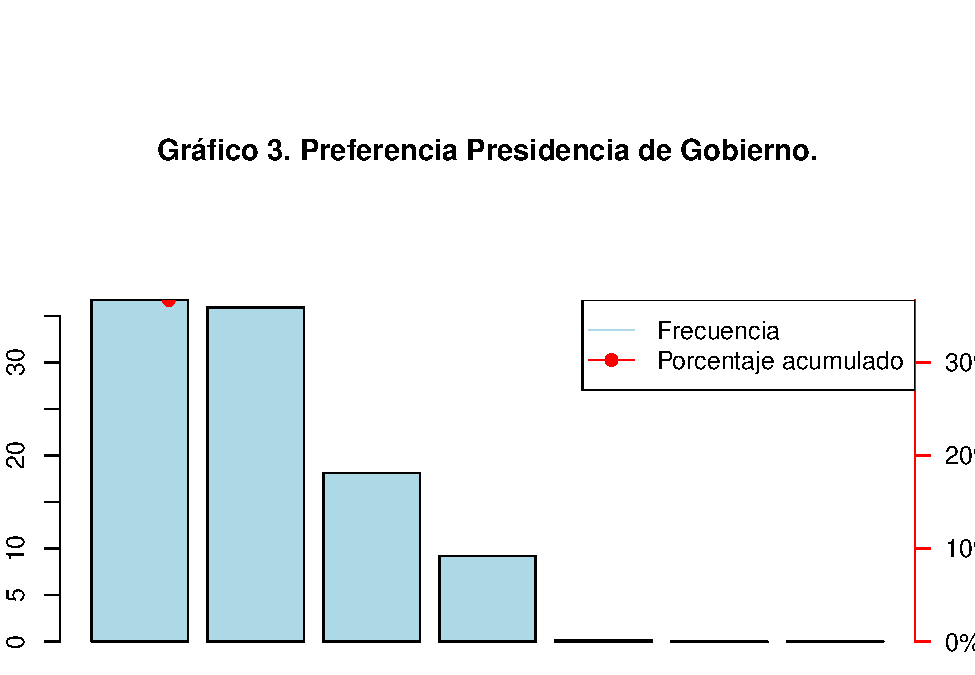
\includegraphics{preferenciaPte_files/figure-latex/graficoPareto-1.pdf}

\newpage

\hypertarget{guardar-resultados-en-fichero-externo}{%
\section{7 GUARDAR RESULTADOS EN FICHERO
EXTERNO}\label{guardar-resultados-en-fichero-externo}}

Los resultados de la tabla de frecuencia se van a guardar en un fichero
externo en al misma carpeta donde hemos guardado los datos fuente
(DATOS).

\begin{Shaded}
\begin{Highlighting}[]
\CommentTok{\# El atributo *output.table* permite exportar los datos a una tabla. }
\NormalTok{df\_tabla}\OtherTok{\textless{}{-}}\NormalTok{grafico}\SpecialCharTok{$}\NormalTok{output.table}

\CommentTok{\# Se redefinen los nombres de campos}
\FunctionTok{colnames}\NormalTok{(df\_tabla)}\OtherTok{\textless{}{-}}\FunctionTok{c}\NormalTok{(}\StringTok{"Frecuencia"}\NormalTok{,}\StringTok{"\%"}\NormalTok{,}\StringTok{"\%\_acumulado"}\NormalTok{, }\StringTok{"\%\_válido"}\NormalTok{,}
                                            \StringTok{"\%\_acumulado válido"}\NormalTok{)}

\CommentTok{\# La función *knitr* mejora el formato de la tabla a mostrar en Rmd}
\FunctionTok{kable}\NormalTok{(df\_tabla,}\AttributeTok{column.width=}\FunctionTok{c}\NormalTok{(}\StringTok{"10\%"}\NormalTok{,}\StringTok{"20\%"}\NormalTok{,}\StringTok{"20\%"}\NormalTok{,}\StringTok{"20\%"}\NormalTok{,}\StringTok{"20\%"}\NormalTok{),}
                    \AttributeTok{caption=}\StringTok{"Tabla de distribución de frecuencias"}\NormalTok{)}
\end{Highlighting}
\end{Shaded}

\begin{longtable}[]{@{}
  >{\raggedright\arraybackslash}p{(\columnwidth - 10\tabcolsep) * \real{0.2692}}
  >{\raggedleft\arraybackslash}p{(\columnwidth - 10\tabcolsep) * \real{0.1410}}
  >{\raggedleft\arraybackslash}p{(\columnwidth - 10\tabcolsep) * \real{0.0769}}
  >{\raggedleft\arraybackslash}p{(\columnwidth - 10\tabcolsep) * \real{0.1538}}
  >{\raggedleft\arraybackslash}p{(\columnwidth - 10\tabcolsep) * \real{0.1154}}
  >{\raggedleft\arraybackslash}p{(\columnwidth - 10\tabcolsep) * \real{0.2436}}@{}}
\caption{Tabla de distribución de frecuencias}\tabularnewline
\toprule\noalign{}
\begin{minipage}[b]{\linewidth}\raggedright
\end{minipage} & \begin{minipage}[b]{\linewidth}\raggedleft
Frecuencia
\end{minipage} & \begin{minipage}[b]{\linewidth}\raggedleft
\%
\end{minipage} & \begin{minipage}[b]{\linewidth}\raggedleft
\%\_acumulado
\end{minipage} & \begin{minipage}[b]{\linewidth}\raggedleft
\%\_válido
\end{minipage} & \begin{minipage}[b]{\linewidth}\raggedleft
\%\_acumulado válido
\end{minipage} \\
\midrule\noalign{}
\endfirsthead
\toprule\noalign{}
\begin{minipage}[b]{\linewidth}\raggedright
\end{minipage} & \begin{minipage}[b]{\linewidth}\raggedleft
Frecuencia
\end{minipage} & \begin{minipage}[b]{\linewidth}\raggedleft
\%
\end{minipage} & \begin{minipage}[b]{\linewidth}\raggedleft
\%\_acumulado
\end{minipage} & \begin{minipage}[b]{\linewidth}\raggedleft
\%\_válido
\end{minipage} & \begin{minipage}[b]{\linewidth}\raggedleft
\%\_acumulado válido
\end{minipage} \\
\midrule\noalign{}
\endhead
\bottomrule\noalign{}
\endlastfoot
Pedro Sánchez & 2631 & 29.9 & 29.9 & 36.7 & 36.7 \\
Alberto Núñez Feijóo & 2576 & 29.3 & 59.2 & 35.9 & 72.6 \\
NA's & 1625 & 18.5 & 100.0 & 0.0 & 100.0 \\
Yolanda Díaz & 1300 & 14.8 & 81.4 & 18.1 & 99.9 \\
Santiago Abascal & 658 & 7.5 & 66.7 & 9.2 & 81.8 \\
Isabel Díaz Ayuso & 8 & 0.1 & 81.5 & 0.1 & 100.0 \\
Ione Belarra & 0 & 0.0 & 81.4 & 0.0 & 99.9 \\
Íñigo Errejón & 0 & 0.0 & 81.4 & 0.0 & 99.9 \\
Total & 8798 & 100.0 & 100.0 & 100.0 & 100.0 \\
\end{longtable}

\hypertarget{fichero-csv-comma-separated-values}{%
\subsection{\texorpdfstring{7.1 Fichero CSV (\emph{Comma-Separated
Values})}{7.1 Fichero CSV (Comma-Separated Values)}}\label{fichero-csv-comma-separated-values}}

Una opción sería crear un fichero \emph{csv}, se trata de un fichero de
texto plano que usa el ``;'' o ``,'' como carácter delimitador de campos
mediante el la función \emph{write.csv} e indicando que la primera fila
contenga el nombre de los campos (row.names = TRUE)

\begin{Shaded}
\begin{Highlighting}[]
\CommentTok{\# Se guarda la tabla de frecuencias en un fichero csv}
\FunctionTok{write.csv}\NormalTok{(grafico, }\AttributeTok{file =} \StringTok{"DATOS/tablafrecResultado.csv"}\NormalTok{,}\AttributeTok{row.names=}\ConstantTok{TRUE}\NormalTok{) }
\end{Highlighting}
\end{Shaded}

\hypertarget{hoja-de-cuxe1lculo-ms-excel-xlsx}{%
\subsection{7.2 Hoja de cálculo MS Excel
(xlsx)}\label{hoja-de-cuxe1lculo-ms-excel-xlsx}}

Una segunda opción sería crear una hoja de cálculo de MS Excel.

\begin{Shaded}
\begin{Highlighting}[]
\CommentTok{\# file= nombre del fichero hoja de cálculo de MSOffice}
\FunctionTok{write.xlsx}\NormalTok{(grafico, }\AttributeTok{file =} \StringTok{"DATOS/tablafrecResultado.xlsx"}\NormalTok{,}
           \AttributeTok{sheetName =} \StringTok{"prefpte"}\NormalTok{, }\AttributeTok{append =} \ConstantTok{FALSE}\NormalTok{)           }
\end{Highlighting}
\end{Shaded}

Alternativamente se puede añadir una nueva página en un fichero excel ya
existente.

\newpage

\hypertarget{id-github}{%
\section{8 EJECUCIÓN DEL Rmd Y REPOSITORIO DE
FICHEROS}\label{id-github}}

Para la ejecución del código R, está disponible el fichero ejecutable
\textbf{preferenciaPte.Rmd} y el fichero de datos
\textbf{datosjulio2023.sav} en el repositorio GitHub. En el mismo
repositorio se encuentra este PDF y un fichero HTML renderizados a
partir del Rmd.

El fichero \emph{datosjulio2023.sav} debe ubicarse en una subcarpeta del
directorio de trabajo con nombre \emph{DATA}.

\begin{longtable}[]{@{}
  >{\centering\arraybackslash}p{(\columnwidth - 4\tabcolsep) * \real{0.2632}}
  >{\raggedright\arraybackslash}p{(\columnwidth - 4\tabcolsep) * \real{0.3684}}
  >{\raggedright\arraybackslash}p{(\columnwidth - 4\tabcolsep) * \real{0.3684}}@{}}
\toprule\noalign{}
\begin{minipage}[b]{\linewidth}\centering

\includegraphics[width=0.1\textwidth,height=\textheight]{../../recursos/iconohyperlink.jpg}
\end{minipage} & \begin{minipage}[b]{\linewidth}\raggedright
\end{minipage} & \begin{minipage}[b]{\linewidth}\raggedright
Enlace a GitHub
\end{minipage} \\
\midrule\noalign{}
\endhead
\bottomrule\noalign{}
\endlastfoot
\href{https://tofermos.github.io/cienciapoliticaygestionpublica/elecciones/estudioCIS3415/DATOS/datosjulio2023.sav}{
\includegraphics[width=0.1\textwidth,height=\textheight]{../../recursos/iconosav.png}}
& Fichero de datos tipo sav &
\href{https://tofermos.github.io/cienciapoliticaygestionpublica/elecciones/estudioCIS3415/DATOS/datosjulio2023.sav}{datosjulio2023.sav} \\
\href{https://tofermos.github.io/cienciapoliticaygestionpublica/elecciones/estudioCIS3415/preferenciaPte.Rmd}{
\includegraphics[width=0.1\textwidth,height=\textheight]{../../recursos/rmarkdown.png}}
& Fichero Rmd &
\href{https://tofermos.github.io/cienciapoliticaygestionpublica/elecciones/estudioCIS3415/preferenciaPte.Rmd}{preferenciaPte.Rmd} \\
\href{https://tofermos.github.io/cienciapoliticaygestionpublica/elecciones/estudioCIS3415/preferenciaPte.html}{
\includegraphics[width=0.1\textwidth,height=\textheight]{../../recursos/iconohtml.png}}
& Fichero HTML &
\href{https://tofermos.github.io/cienciapoliticaygestionpublica/elecciones/estudioCIS3415/preferenciaPte.html}{preferenciaPte.html} \\
\href{https://tofermos.github.io/cienciapoliticaygestionpublica/elecciones/estudioCIS3415/probabilidadVoto.pdf}{
\includegraphics[width=0.1\textwidth,height=\textheight]{../../recursos/iconopdf.png}}
& Fichero PDF &
\href{https://tofermos.github.io/cienciapoliticaygestionpublica/elecciones/estudioCIS3415/probabilidadVoto.pdf}{preferenciaPte.pdf} \\
\href{https://tofermos.github.io/cienciapoliticaygestionpublica/}{
\includegraphics[width=0.2\textwidth,height=\textheight]{../../recursos/iconogithub.png}}
& &
\href{https://tofermos.github.io/cienciapoliticaygestionpublica/}{Repositorio
tofermos} \\
\end{longtable}

\end{document}
